% Foliensatz: "AFu-Kurs nach DJ4UF" von DK0TU, Amateurfunkgruppe der TU Berlin
% Lizenz: CC BY-NC-SA 3.0 de (http://creativecommons.org/licenses/by-nc-sa/3.0/de/)
% Autoren:
% Felix Baum DB4UM <baum@campus.tu-berlin.de>
% Lars Weiler <dc4lw@darc.de>

\documentclass[aspectratio=169]{beamer}

\usepackage[ngerman]{babel} % deutsche Worttrennung etc.
\usepackage[utf8]{inputenc} % UTF8 Text

\usepackage[super, comma, numbers, square, sort]{natbib}

\usepackage{hyperref}       % Hyperref Package für bessere Referenzen (todo)
\hypersetup{
	colorlinks=false,       %   false: boxed links; true: colored links
    %linkcolor=white,       %   color of internal links (change box color with linkbordercolor)
    citecolor=red,          %   color of links to bibliography
    filecolor=white,        %   color of file links
    urlcolor=blue           %   color of external links
}

\usepackage{multirow}
\usepackage{wasysym}  % Math Symbols like \permil
%\usepackage{colortbl}
%\usepackage{subscript}
%\usepackage{caption}
%\usepackage{setspace}
%\usepackage{xcolor}        % benutze CodeListe

% Footnote
%\usepackage{hanging}
%
%\setbeamertemplate{footnote}{%
%  \hangpara{2em}{1}%
%  \makebox[2em][l]{\insertfootnotemark}\footnotesize\insertfootnotetext\par%
%}


%\usepackage{pgf}
%\usepackage{tikz}
%\usetikzlibrary{arrows,automata}
%\usetikzlibrary{positioning}
%
%\tikzset{
%    state/.style={
%           rectangle,
%           rounded corners,
%           draw=black, very thick,
%           minimum height=2em,
%           minimum width=2pt,
%           inner sep=2pt,
%           text centered,
%           },
%}

%\usepackage{listings}
%\lstset{basicstyle=\small, numberstyle=\tiny, extendedchars=true, numbers=left, numbersep=5pt}
%\lstset{showtabs=false, showspaces=false, showstringspaces=false}
%%\lstset{backgroundcolor=\color{white!75!lightgray}, , frame=single}
%%\lstset{backgroundcolor=\color{white}}
%%\lstset{backgroundcolor=none}
%\lstset{keywordstyle=\color{blue!50!gray},  identifierstyle=\color{black}}
%\lstset{commentstyle=\color{green!50!gray}, stringstyle=\color{red!50!gray}}
%\lstset{language=C, fontadjust=true, tabsize=2, breaklines=true}
%\lstset{backgroundcolor=\color{white!75!lightgray}, caption=\lstname, frame=single}
%\lstset{emphstyle=\color{black}\fbox}
%
%% Keine "Listing:"-Caption
%\captionsetup{labelformat=empty,labelsep=none}
%
%% für mathematische Umgebungen
%\usepackage{amsmath,amsfonts,amssymb}
%
%\lstdefinestyle{Bash}{
%language=Bash,
%frame=single,
%rulecolor=\color{black},
%backgroundcolor=\color{gray!50},
%keywordstyle=\color{black},
%identifierstyle=,
%commentstyle=\color{black},
%stringstyle=\color{magenta!65!white},
%showstringspaces=false,
%basicstyle=\footnotesize\ttfamily\color{black},
%numbers=none,
%breaklines=true,
%captionpos=b
%}

%\usepackage{listings}
%
%\lstdefinestyle{basic}{
%    captionpos=t,%
%    basicstyle=\footnotesize\ttfamily,%
%    numberstyle=\tiny,%
%    numbers=left,%
%    stepnumber=1,%
%    frame=single,%
%    showspaces=false,%
%    showstringspaces=false,%
%    showtabs=false,%
%    %
%    keywordstyle=\color{blue},%
%    identifierstyle=,%
%    commentstyle=\color{gray},%
%    stringstyle=\color{magenta}%
%}



% fließende Boxen haben keinen Abstand
%\fboxsep0mm

% inkludiere Creative Commons Helper
%%%%%%%%%%%%%%%%%%%%%%%%%%%%%%%%%%%%%%%%%%%%%%%%%%%%%%%%%%%%%%%%
%% ccBeamer 0.1, 2007-07-02                                   %%
%% Written by Sebastian Pipping <webmaster@hartwork.org>      %%
%% ---------------------------------------------------------- %%
%% Licensed under Creative Commons Attribution-ShareAlike 3.0 %%
%% http://creativecommons.org/licenses/by-sa/3.0/             %%
%%%%%%%%%%%%%%%%%%%%%%%%%%%%%%%%%%%%%%%%%%%%%%%%%%%%%%%%%%%%%%%%


%% Images
\newcommand{\CcImageBy}[1]{%
	
\includegraphics[scale=#1]{texdata/creative_commons/cc_by_30.pdf}%
}
\newcommand{\CcImageCc}[1]{%
	
\includegraphics[scale=#1]{texdata/creative_commons/cc_cc_30.pdf}%
}
\newcommand{\CcImageDevNations}[1]{%
	
\includegraphics[scale=#1]{texdata/creative_commons/cc_dev_nations_30.pdf}%
}
\newcommand{\CcImageNc}[1]{%
	
\includegraphics[scale=#1]{texdata/creative_commons/cc_nc_30.pdf}%
}
\newcommand{\CcImageNd}[1]{%
	
\includegraphics[scale=#1]{texdata/creative_commons/cc_nd_30.pdf}%
}
\newcommand{\CcImagePd}[1]{%
	
\includegraphics[scale=#1]{texdata/creative_commons/cc_pd_30.pdf}%
}
\newcommand{\CcImageSa}[1]{%
	
\includegraphics[scale=#1]{texdata/creative_commons/cc_sa_30.pdf}%
}
\newcommand{\CcImageSampling}[1]{%
	
\includegraphics[scale=#1]{texdata/creative_commons/cc_sampling_30.pdf}%
}
\newcommand{\CcImageSamplingPlus}[1]{%
	
\includegraphics[scale=#1]{texdata/creative_commons/cc_sampling_plus_30.pdf}%
}


%% Groups
\newcommand{\CcGroupBy}[2]{% zoom, gap
	\CcImageCc{#1}\hspace*{#2}\CcImageBy{#1}%
}
\newcommand{\CcGroupByNc}[2]{% zoom, gap
	\CcImageCc{#1}\hspace*{#2}\CcImageBy{#1}\hspace*{#2}\CcImageNc{#1}%
}
\newcommand{\CcGroupByNcNd}[2]{% zoom, gap
	\CcImageCc{#1}\hspace*{#2}\CcImageBy{#1}\hspace*{#2}\CcImageNc{#1}\hspace*{#2}\CcImageNd{#1}%
}
\newcommand{\CcGroupByNcSa}[2]{% zoom, gap
	\CcImageCc{#1}\hspace*{#2}\CcImageBy{#1}\hspace*{#2}\CcImageNc{#1}\hspace*{#2}\CcImageSa{#1}%
}
\newcommand{\CcGroupByNd}[2]{% zoom, gap
	\CcImageCc{#1}\hspace*{#2}\CcImageBy{#1}\hspace*{#2}\CcImageNd{#1}%
}
\newcommand{\CcGroupBySa}[2]{% zoom, gap
	\CcImageCc{#1}\hspace*{#2}\CcImageBy{#1}\hspace*{#2}\CcImageSa{#1}%
}
\newcommand{\CcGroupDevNations}[2]{% zoom, gap
	\CcImageCc{#1}\hspace*{#2}\CcImageDevNations{#1}%
}
\newcommand{\CcGroupNcSampling}[2]{% zoom, gap
	\CcImageCc{#1}\hspace*{#2}\CcImageNc{#1}\hspace*{#2}\CcImageSampling{#1}%
}
\newcommand{\CcGroupPd}[1]{% zoom
	\CcImagePd{#1}%
}
\newcommand{\CcGroupSampling}[1]{% zoom
	\CcImageSampling{#1}%
}
\newcommand{\CcGroupSamplingPlus}[1]{% zoom
	\CcImageSamplingPlus{#1}%
}


%% Text
\newcommand{\CcLongnameBy}{Attribution}
\newcommand{\CcLongnameByNc}{Attribution-NonCommercial}
\newcommand{\CcLongnameByNcNd}{Attribution-NoDerivs}
\newcommand{\CcLongnameByNcSa}{Attribution-NonCommercial-ShareAlike}
\newcommand{\CcLongnameByNd}{Attribution-NoDerivs}
\newcommand{\CcLongnameBySa}{Attribution-ShareAlike}

\newcommand{\CcNote}[1]{% longname
	This work is licensed under the \textit{Creative Commons #1 3.0 License}.%
}


% generelles Thema auswählen
\usetheme{Goettingen} %Berlin spart ohne Sidebar allerdings angenehm Platz
% AnnArbor | Antibes | Bergen | Berkeley | Berlin | Boadilla | boxes | CambridgeUS | Copenhagen | Darmstadt | default | Dresden | Frankfurt | Goettingen | Hannover | Ilmenau | JuanLesPins | Luebeck | Madrid | Malmoe | Marburg | Montpellier | PaloAlto | Pittsburgh | Rochester | Singapore | Szeged | Warsaw

% Farben wählen
\usecolortheme{beetle}
% beaver | beetle | crane | default | dolphin | dove | fly | lily | orchid | rose | seagull | seahorse | sidebartab | structure | whale | wolverine

% Setze alle Farben auf Grau und Weiß
%\definecolor{craneorange}{RGB}{64,64,64}
%\definecolor{craneblue}{RGB}{255,255,255}

% Schriftart wählen
\usefonttheme{default}
% default | professionalfonts | serif | structurebold | structureitalicserif | structuresmallcapsserif

% Innere Themen(Kopf-, Fuß-, Sidebar usw)
%\useinnertheme{default}
\useinnertheme{circles}
% default | inmargin | rectangles | rounded | circles

% Äußere Themen (Anordnung der inneren, grenzen der Folien etc.)
\useoutertheme{infolines}
% default | infolines | miniframes | shadow | sidebar | smoothbars | smoothtree | split | tree

% Deaktiviere Navigations-Symbole ({} -> leer)
\setbeamertemplate{navigation symbols}{}
%\setbeamertemplate{navigation symbols}{\large \ifnum \insertframenumber <10 0\fi\insertframenumber/\inserttotalframenumber\vspace*{0.2ex}}

% Zeige ein Hintergrundbild
\setbeamertemplate{background canvas}{
        \hspace*{-2.0cm}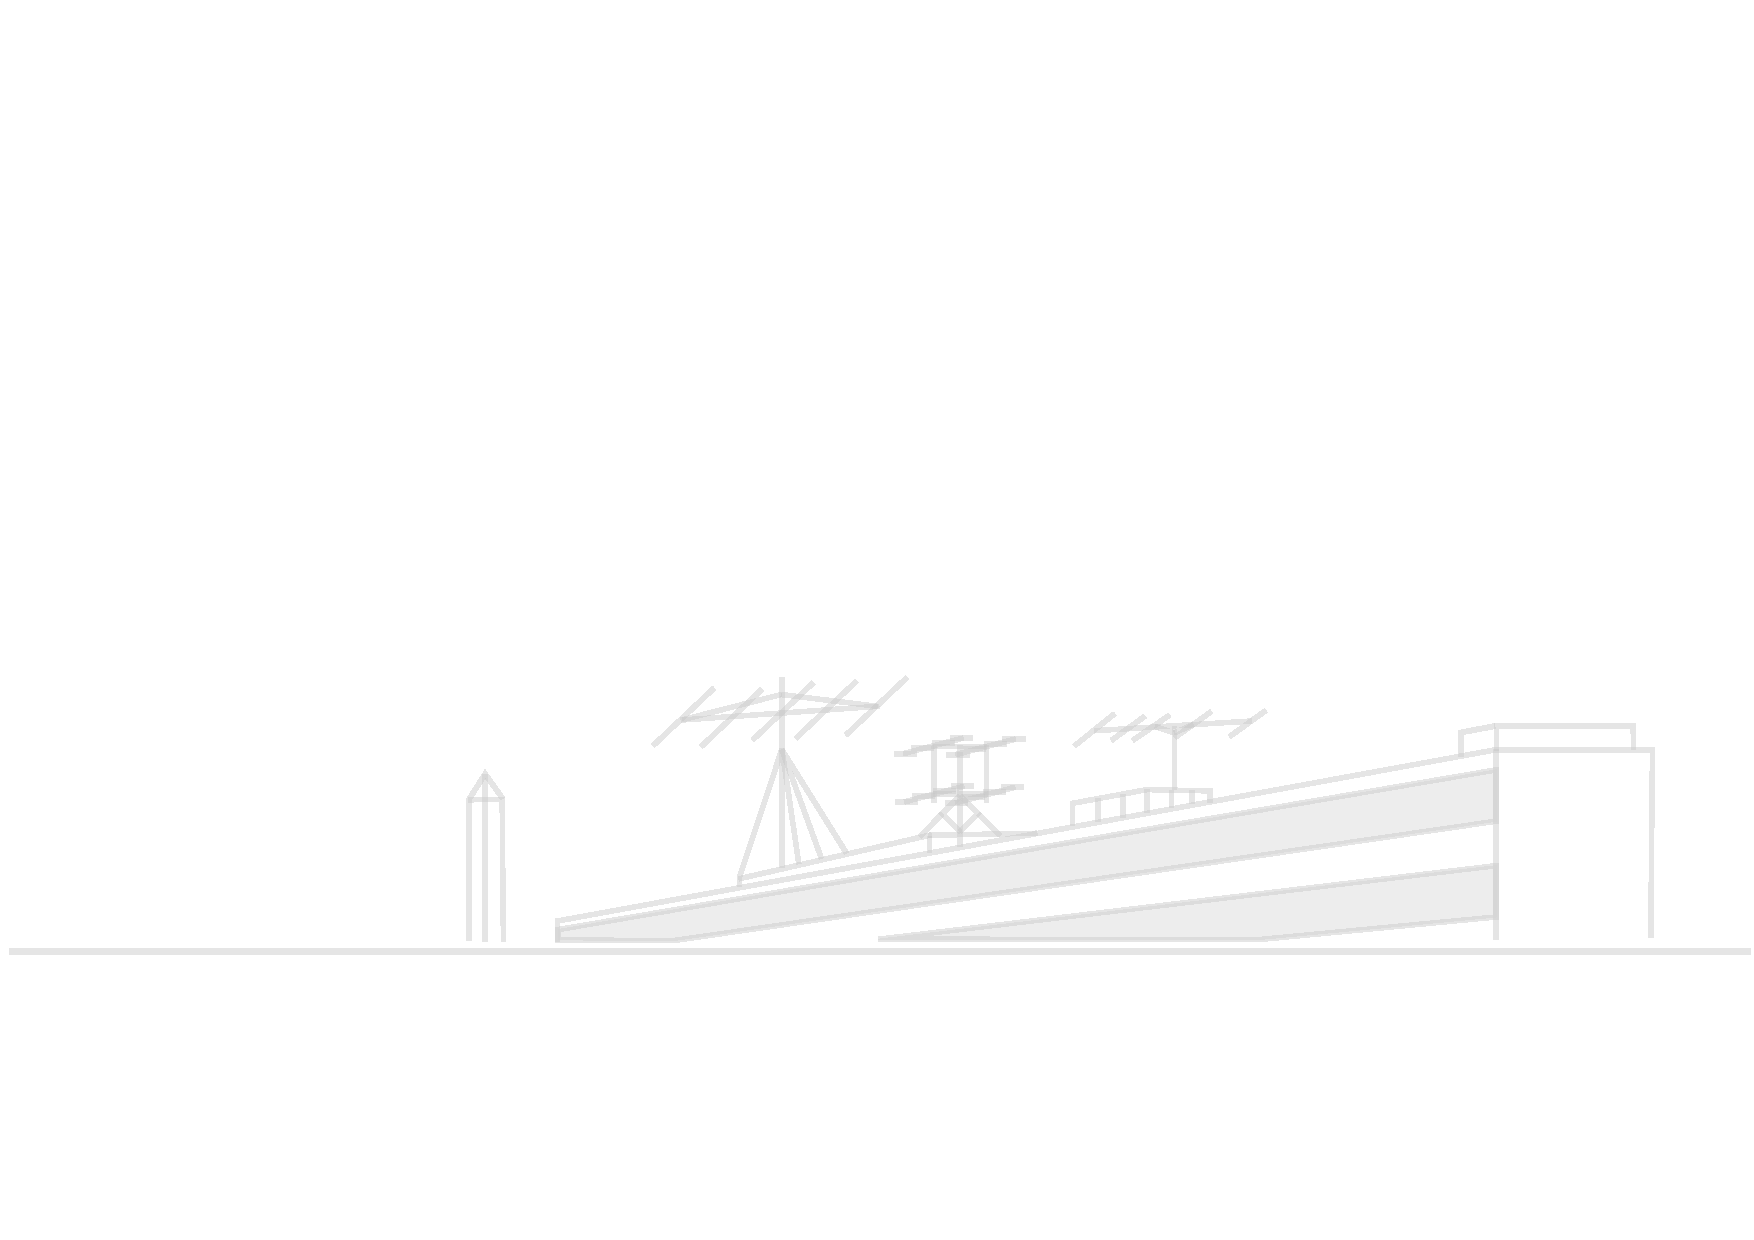
\includegraphics[width=17.8cm]{texdata/dk0tu_rooftop_background.pdf}
}

% Foliennummer einfügen
\setbeamertemplate{footline}[frame number]
%\setbeamertemplate{footline}{}

% Ändere das Zeichen vor jedem item
%\setbeamertemplate{itemize item}{\color{craneorange}$\blacktriangleright$}
%\setbeamertemplate{itemize subitem}{\color{craneorange}$\triangleright$}
%\setbeamertemplate{itemize subsubitem}{\color{craneorange}$\blacktriangleright$}

% Ändert die Blöcke 
\setbeamertemplate{blocks}[rounded][shadow=true]
% default | rounded [shadow=true|false]

%
% Eigene Kommandos
%

% Hack to get natbib and beamer working together. "The beamer user guide suggests
% that only the manual bibliography entry approach is supported"
% on some system it works out of the box, sometimes you need the hack :-(
% so check it --dl7bst
\ifdefined\newblock
    \relax
\else
    \newcommand{\newblock}{}
\fi

% \includedia command to generate png out of a dia file
% NEEDS installed dia and pdflatex option --shell-escape
\newcommand{\includedia}[1]{
    \immediate\write18{/usr/bin/dia #1.dia -e #1_diatmp.png -t png}
}

% RICHIG GROSSER FONT!
\newfont{\bigfont}{cmr10 at 144pt}
\newfont{\smallfont}{cmr10 at 8pt}

% Römische Ziffern
\makeatletter
\newcommand{\rmnum}[1]{\romannumeral #1}
\newcommand{\Rmnum}[1]{\expandafter\@slowromancap\romannumeral #1@}
\makeatother

% Schwarze Überschrift
%\setbeamercolor{frametitle}{fg=black}
%\setbeamercolor{title}{fg=black}

% Item- und Box-Farben
\definecolor{deepBlue}{HTML}{000066}
\setbeamercolor{itemize item}{fg=deepBlue}
\setbeamercolor{itemize subitem}{fg=deepBlue}
\setbeamercolor{description item}{fg=deepBlue}
\setbeamercolor{block title}{fg=deepBlue!100, bg=blue!15}
\setbeamercolor{block body}{fg=black, bg=blue!5}
\setbeamercolor{block title alerted}{fg=deepBlue, bg=red!75}
\setbeamercolor{block body alerted}{fg=black, bg=red!15}
\setbeamercolor*{block title example}{fg=blue!50, bg=blue!10}
\setbeamercolor*{block body example}{fg= blue, bg=blue!5}

%\setbeamercolor{section in head/foot}{parent=palette primary}
%\setbeamercolor{subsection in head/foot}{parent=palette secondary}
%\setbeamercolor{sidebar}{fg=darkblue,bg=yellow!90!orange}
%\setbeamercolor{title in sidebar}{fg=darkblue}
%\setbeamercolor{author in sidebar}{fg=darkblue}
%\setbeamercolor{section in sidebar}{fg=darkblue!10!black}
%\setbeamercolor{subsection in sidebar}{fg=darkblue!50!black}

% Titlepage Infos
\title{AFu-Kurs nach DJ4UF}
\author[DKØTU]{DKØTU\\ \footnotesize{Amateurfunkgruppe der TU Berlin}}
\institute[DKØTU]{\url{http://www.dk0tu.de} }

% PDF-Eigenschaften
\subject{DK0TU-Amateurfunkkurs nach DJ4UF}
\keywords{Amateurfunk Kurs HAM Radio Course CC-BY-NC-SA OpenSource TU Berlin DK0TU}

\subtitle{Technik A05: \\
  Die Diode und ihre Anwendungen \\[2em]}
\date{Stand 04.05.2017}
 \begin{document}

\begin{frame}
    \titlepage
    \vfill
    \begin{center}
        \ccbyncsaeu\\
        {\tiny This work is licensed under the \em{Creative Commons Attribution-NonCommercial-ShareAlike 3.0 License}.}\\[0.5ex]
         \tiny Amateurfunkgruppe der Technische Universität Berlin (AfuTUB), DKØTU
         %\includegraphics[scale=0.5]{img/DK0TU_Logo.pdf}
    \end{center}
\end{frame}


\section*{Wiederholung}

\begin{frame}
  \frametitle{Halbleiter}
  \begin{itemize}
    \item Was ist ein Halbleiter? (Erinnern aus alter Technik)
    \item Wann leitet eine Siliziumdiode?
    \item Wann leitet eine Germaniumdiode?
    \item Was bedeutet p-dotiert?
  \end{itemize}
\end{frame}

\begin{frame}
  \frametitle{Leitet die Siliziumdiode?}
  \begin{center}
    \begin{figure}
      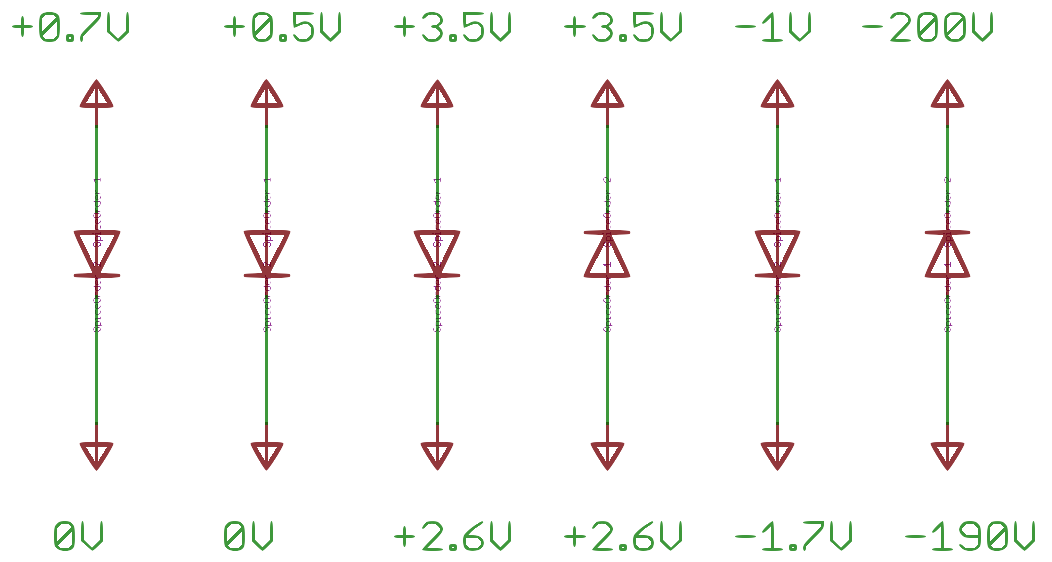
\includegraphics[width=1\textwidth,height=.75\textheight,keepaspectratio]{a05/Leit_Diode.png}
      \caption{Leitende und nicht leitende Dioden}
    \end{figure}
  \end{center}
\end{frame}

\begin{frame}
  \frametitle{Diode Raumladungszone}
  \begin{center}
    \begin{figure}
      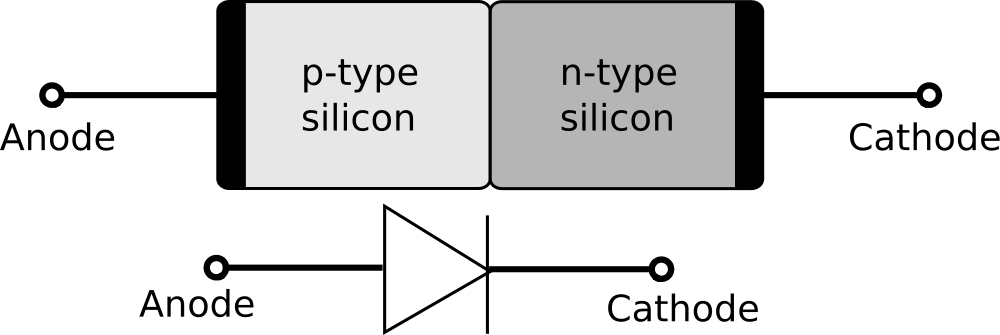
\includegraphics[width=1\textwidth,height=.6\textheight,keepaspectratio]{a05/diode_with_electrical_symbol.png}
      \attribcaption{Raumladungszone}{Raffamaiden}{https://commons.wikimedia.org/wiki/File:PN_diode_with_electrical_symbol.svg}{\ccbysa}
    \end{figure}
    \large Wie, wo und warum bildet sich eine Raumladungszone (RLZ), auch Verarmungszone genannt, in der pn-Diode aus?
  \end{center}
\end{frame}

\begin{frame}
  \frametitle{Leitet die Siliziumdiode?}
  \begin{center}
    \begin{figure}
      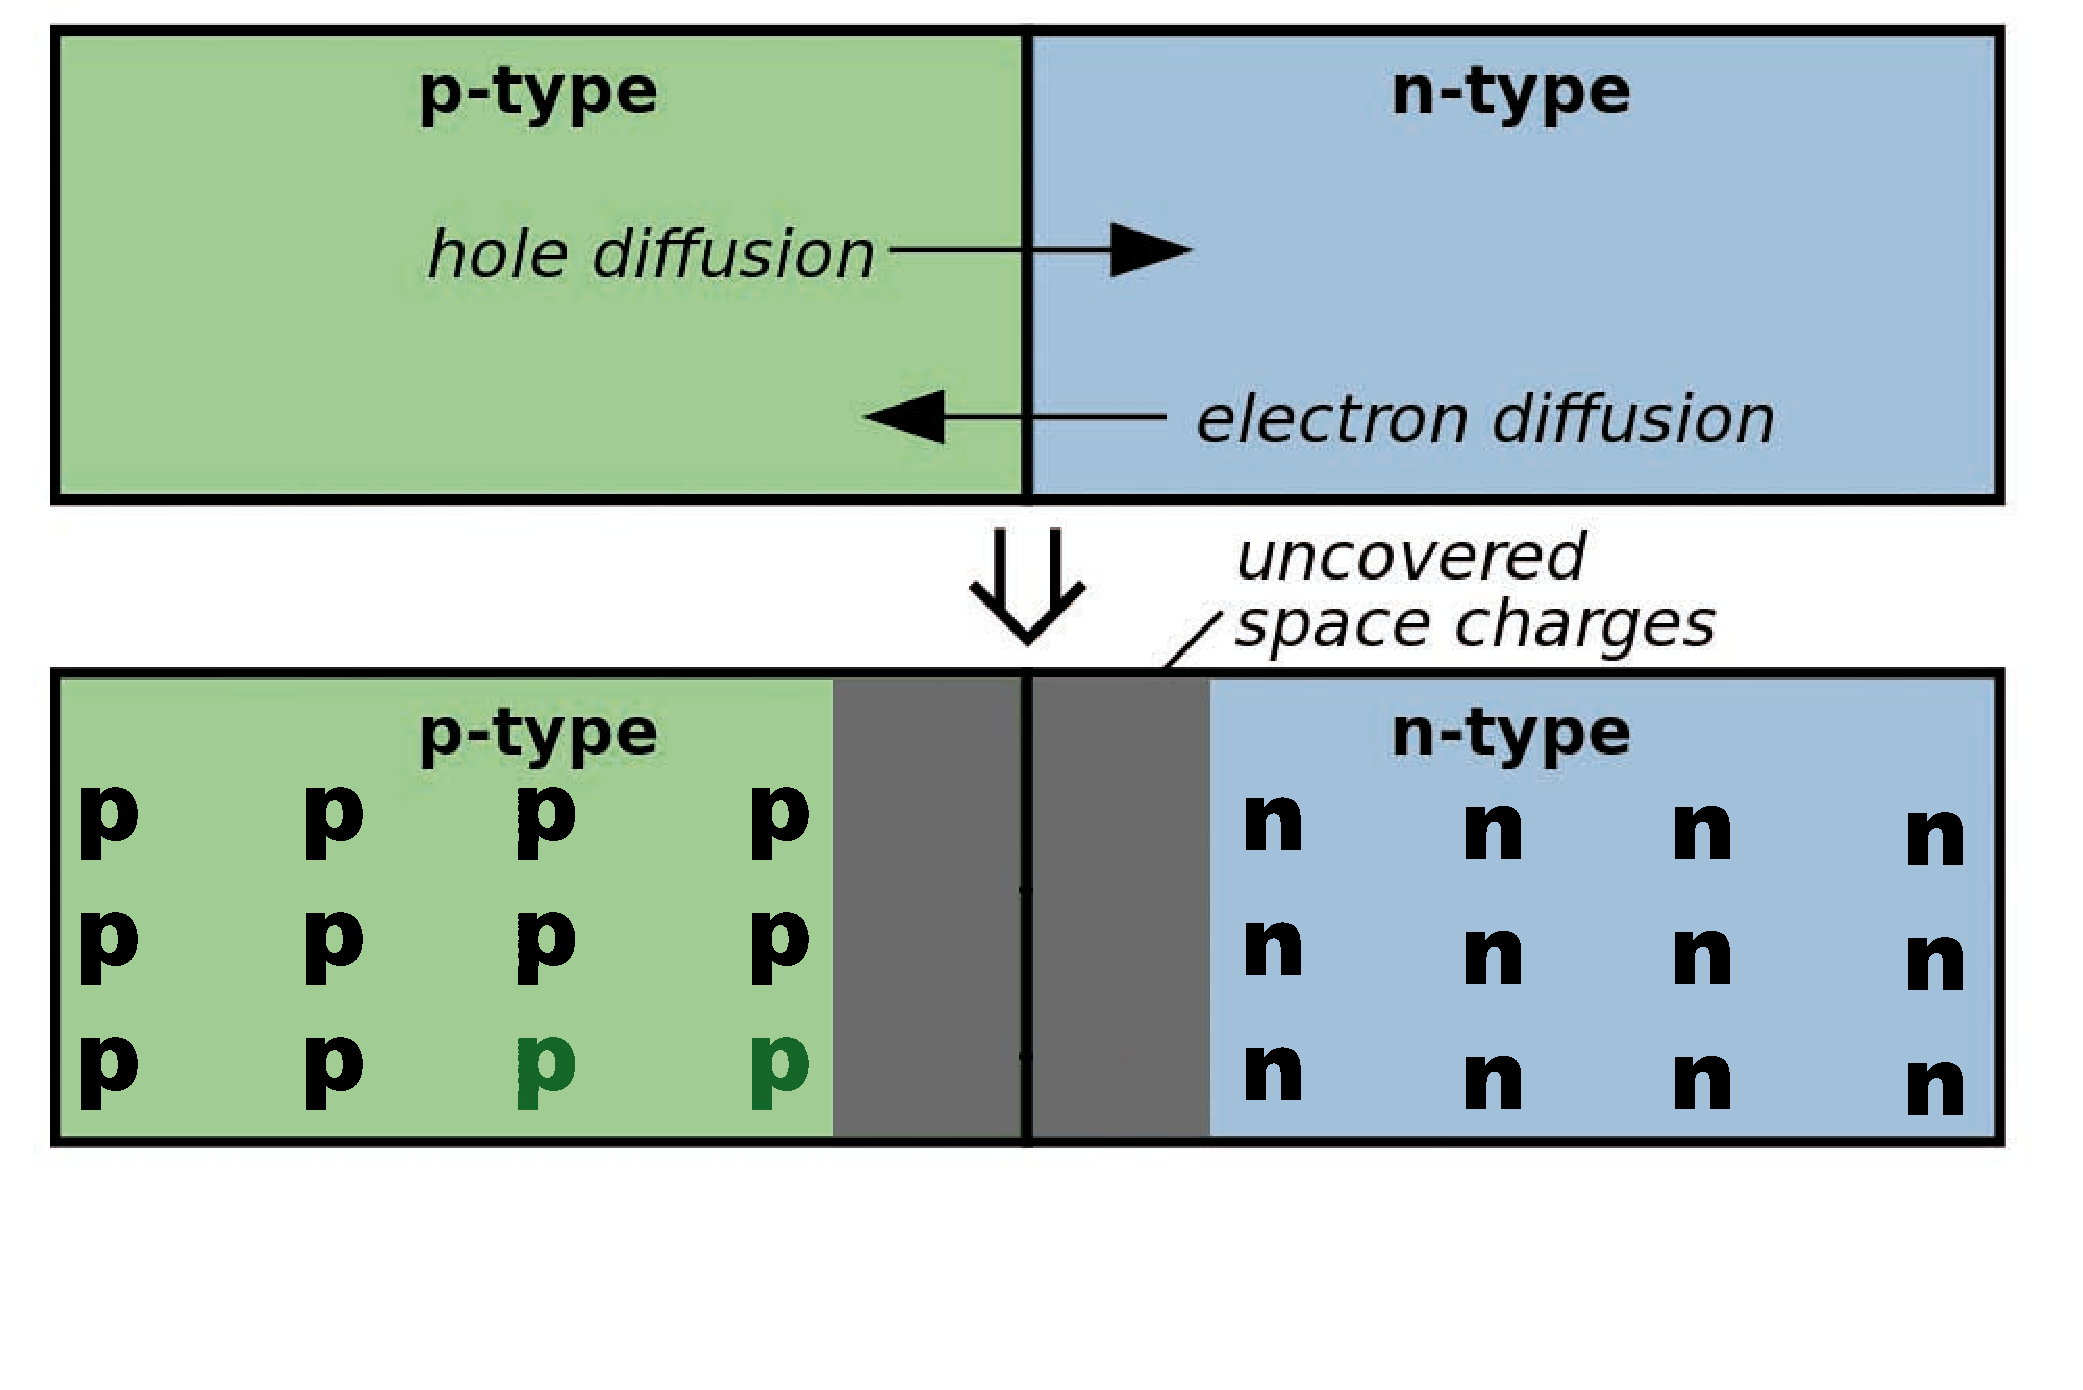
\includegraphics[width=1\textwidth,height=.5\textheight,keepaspectratio]{a05/Pn_Junction_Diffusion_and_Drift.pdf}
      \attribcaption{Diffusionsstrom}{Inductiveload}{https://commons.wikimedia.org/wiki/File:Pn_Junction_Diffusion_and_Drift.svg}{\ccpd}
    \end{figure}
    \emph{Durch Ausgleichsbewegungen (Diffusionsstrom) zwischen dem p- und dem n-Gebiet wird die RLZ gebildet.\\
    Dort gibt es keine frei beweglichen Ladungsträger mehr.}
  \end{center}
\end{frame}

\begin{frame}
  \frametitle{Diodenkennlinien}
  \begin{columns}[c]
    \column[c]{.5\textwidth}
    \begin{figure}
      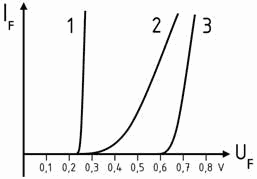
\includegraphics[width=1\textwidth,height=.85\textheight,keepaspectratio]{a05/tc511.png}
      \caption{Prüfungsfrage TC511}
    \end{figure}
    \column{.45\textwidth}
    Welcher Diodentyp hat welche Kennlinie?
    \begin{description}
      \item[1 $\rightarrow$] \only<2>{Schottkydiode}
      \item[2 $\rightarrow$] \only<2>{Germaniumdiode}
      \item[3 $\rightarrow$] \only<2>{Siliziumdiode}
    \end{description}
  \end{columns}
\end{frame}

\section*{Verschiedene Spezialdioden}

\subsection*{Schottky-Diode}
\begin{frame}
  \frametitle{Schottky-Diode}
  \begin{columns}[c]
    \column[c]{.5\textwidth}
    \begin{center}
      \begin{figure}
        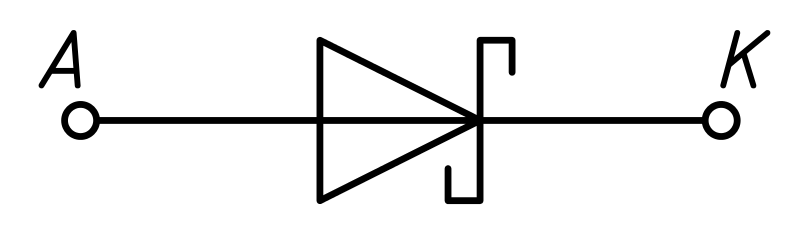
\includegraphics[width=1\textwidth,height=.1\textheight,keepaspectratio]{a05/Diode-Schottky-EN_A-K.png}
        \attribcaption{Schaltzeichen einer Schottky-Diode}{GregorioW}{https://commons.wikimedia.org/wiki/File:Diode-Schottky-EN_A-K.svg?uselang=de}{\ccbysa}
      \end{figure}
      \begin{figure}
        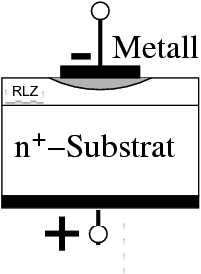
\includegraphics[width=0.8\textwidth,height=.4\textheight,keepaspectratio]{a05/AusfuerungsformenSchottkyDiode.png}
        \attribcaption{Ausführungsformen einer Schottky-Diode}{Patrick-Emil Zörner}{http://commons.wikimedia.org/wiki/File:AusfuerungsformenSchottkyDiode.png}{\ccbysa}
      \end{figure}
    \end{center}
    \column{.45\textwidth}
    \begin{itemize}
      \item Sehr gut geeignet für HF-Schaltungen
      \item Raumladungszone baut sich schneller auf und ab
      \item RLZ zwischen Metall und N-gebiet
      \item Geringe Durchlassspannung ($0.25V$)
    \end{itemize}
  \end{columns}
\end{frame}

\subsection*{Kapazitätsdiode}
\begin{frame}
  \frametitle{Kapazitätsdiode}
  \begin{columns}[c]
    \column[c]{.5\textwidth}
    \begin{center}
      \begin{figure}
        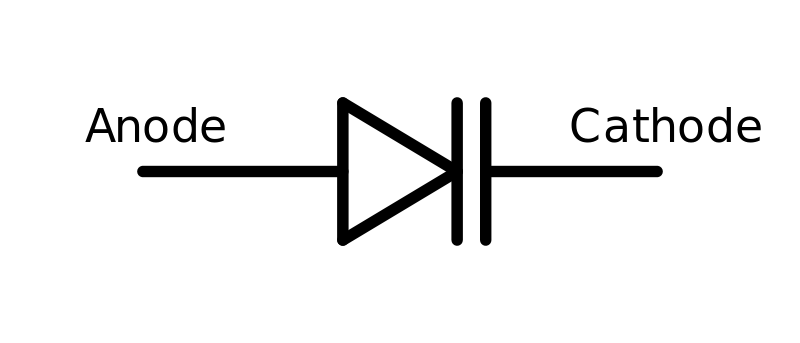
\includegraphics[width=1\textwidth,height=.15\textheight,keepaspectratio]{a05/Varicap_symbol.png}
        \attribcaption{Schaltzeichen Varicap}{Omegatron}{http://commons.wikimedia.org/wiki/File:Varicap_symbol.svg}{\ccbysa}
      \end{figure}
      \begin{figure}
        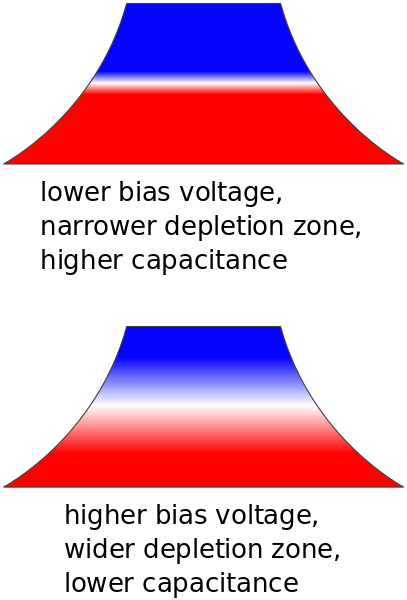
\includegraphics[width=0.8\textwidth,height=.4\textheight,keepaspectratio]{a05/Varactor_function.png}
        \attribcaption{Funktion Varicap}{Shaddack}{https://commons.wikimedia.org/wiki/File:Varactor_function.svg}{\ccpd}
      \end{figure}
    \end{center}
    \column{.45\textwidth}
    \begin{itemize}
      \item auch \emph{Varicap}, \emph{Varaktor} oder \emph{Abstimmdiode}
      \item Kapazität sinkt mit steigender Spannung
      \item in fast allen VCOs verbaut
    \end{itemize}
  \end{columns}
\end{frame}

\subsection*{Z-Diode}
\begin{frame}
  \frametitle{Z-Diode}
  \begin{columns}[c]
    \column[c]{.5\textwidth}
    \begin{center}
      \begin{figure}
        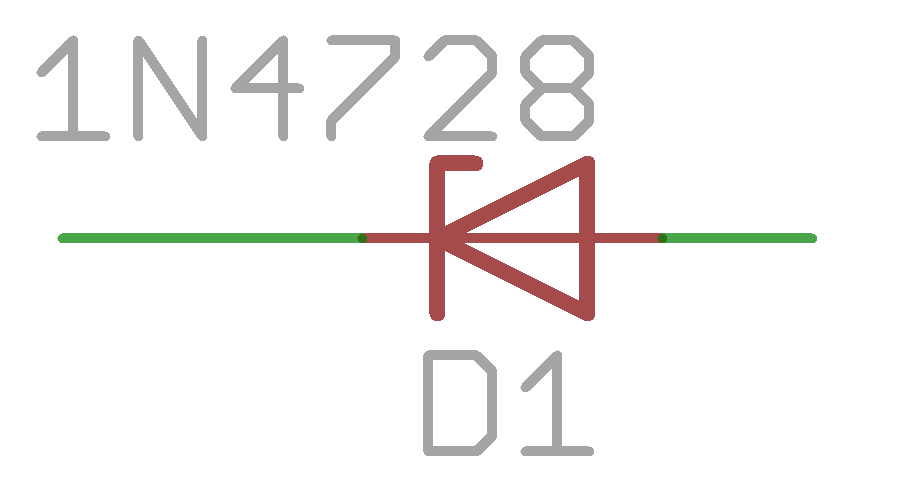
\includegraphics[width=.8\textwidth,height=.3\textheight,keepaspectratio]{a05/z-diode.png}
        \caption{Schaltzeichen Z-Diode}
      \end{figure}
    \end{center}
    \column{.45\textwidth}
    \begin{itemize}
      \item Meist zur Spannungsstabilisierung
      \item Einbau in Sperrichtung
      \item Zur Sicherheit immer mit Vorwiderstand einbauen
    \end{itemize}
  \end{columns}
\end{frame}

\begin{frame}
  \frametitle{Z-Diode}
  \begin{center}
    \begin{figure}
      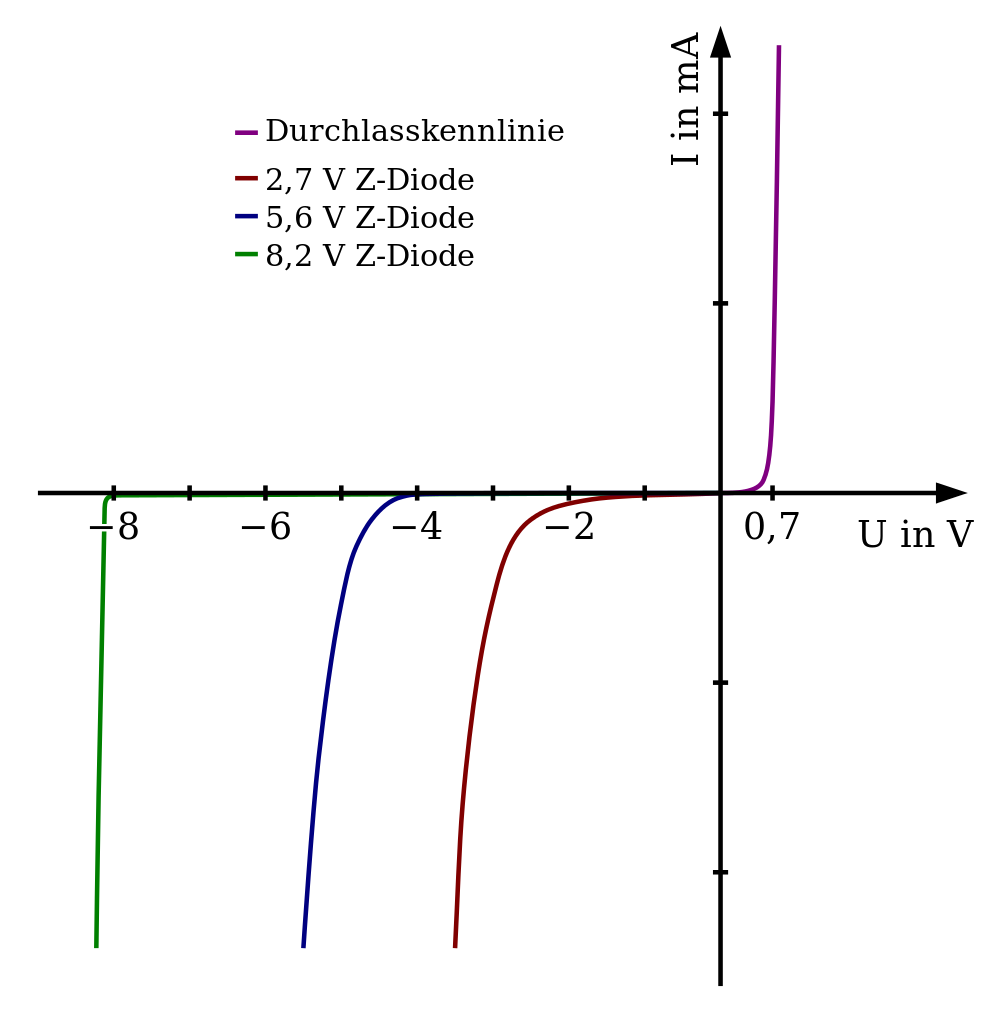
\includegraphics[width=.7\textwidth,height=.75\textheight,keepaspectratio]{a05/Kennlinie_Z-Diode.png}
      \attribcaption{Kennlinie Z-Diode}{Biezl}{https://commons.wikimedia.org/wiki/File:Kennlinie_Z-Diode.svg}{\ccpd}
    \end{figure}
  \end{center}
\end{frame}

\subsection*{Fotodiode}
\begin{frame}
  \frametitle{Fotodiode}
  \begin{columns}[c]
    \column[c]{.5\textwidth}
    \begin{center}
      \begin{figure}
        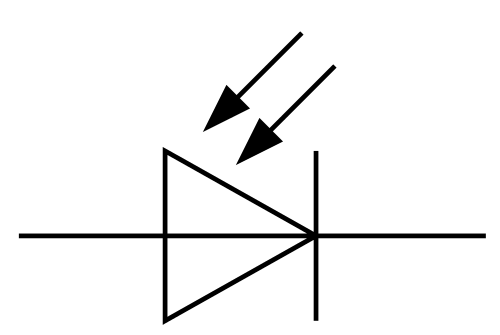
\includegraphics[width=1\textwidth,height=.15\textheight,keepaspectratio]{a05/Symbol_Photodiode.png}
        \attribcaption{Schaltzeichen Photodiode}{MovGP0}{https://commons.wikimedia.org/wiki/File:Symbol_Photodiode.svg}{\ccpd}
      \end{figure}
      \begin{figure}
        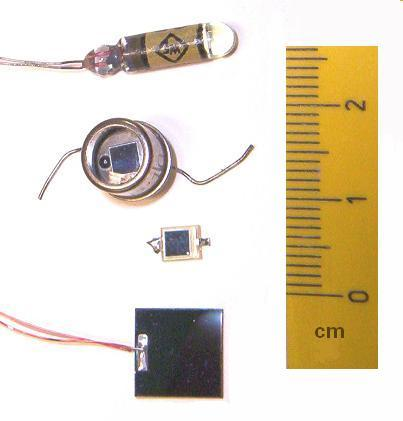
\includegraphics[width=0.8\textwidth,height=.4\textheight,keepaspectratio]{a05/Fotodio.jpg}
        \attribcaption{Verschiedene Si-Fotodioden, oben eine Ge-Fotodiode}{Ulfbastel}{https://commons.wikimedia.org/wiki/File:Fotodio.jpg}{\ccbysa}
      \end{figure}
    \end{center}
    \column{.45\textwidth}
    \begin{itemize}
      \item Ändert Widerstand abhängig von Lichteinfall
      \item Wird z.B. als Helligkeitssensor verwendet
    \end{itemize}
  \end{columns}
\end{frame}

\subsection*{Solarzelle}
\begin{frame}
  \frametitle{Solarzelle}
  \begin{center}
    \begin{figure}
      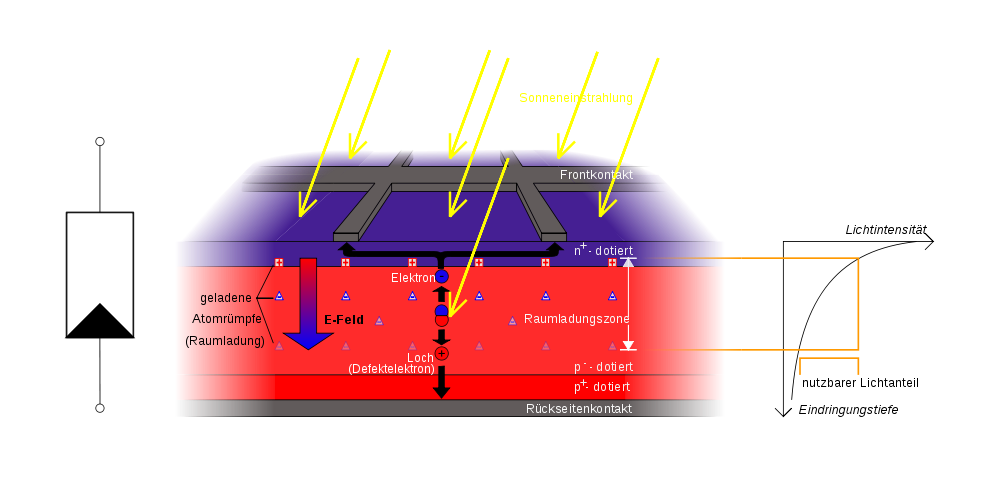
\includegraphics[width=1\textwidth,height=.75\textheight,keepaspectratio]{a05/Solarzelle_Funktionsprinzip2.png}
      \attribcaption{Entscheidend für das Verständnis ist ein elektrisches Feld, das im Material ständig vorhanden ist.}{Degreen}{https://commons.wikimedia.org/wiki/File:Solarzelle_Funktionsprinzip2.svg}{\ccbysa}
    \end{figure}
  \end{center}
\end{frame}

\begin{frame}
  \frametitle{Kennlinie Solar + Fotodiode}
  \begin{center}
    \begin{figure}
      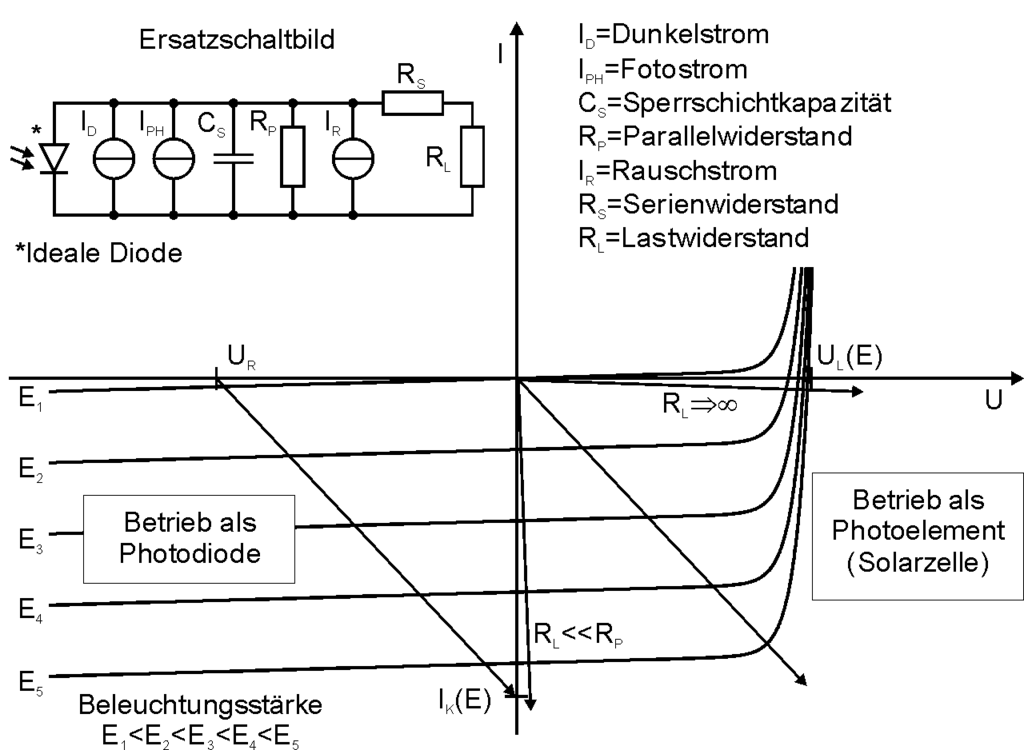
\includegraphics[width=1\textwidth,height=.75\textheight,keepaspectratio]{a05/Kennlinie_Photodiode_1.png}
      \attribcaption{Kennlinie einer Photodiode}{Gregor Hess (Ghe42)}{https://commons.wikimedia.org/wiki/File:Kennlinie_Photodiode_1.png}{\ccbysa}
    \end{figure}
  \end{center}
\end{frame}

\subsection*{LED}
\begin{frame}
  \frametitle{Leuchtdiode (LED)}
  \begin{columns}[c]
    \column[c]{.5\textwidth}
    \begin{center}
      \begin{figure}
        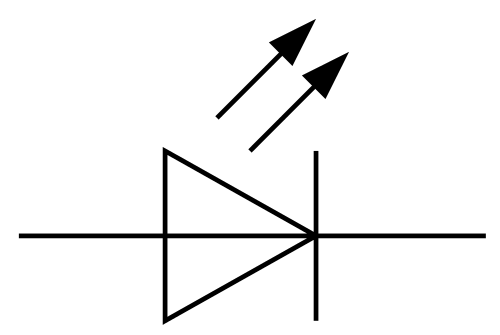
\includegraphics[width=1\textwidth,height=.15\textheight,keepaspectratio]{a05/Symbol_LED.png}
        \attribcaption{Schaltzeichen einer Leuchtdiode}{MovGP0}{https://commons.wikimedia.org/wiki/File:Symbol_LED.svg}{\ccpd}
      \end{figure}
      \begin{figure}
        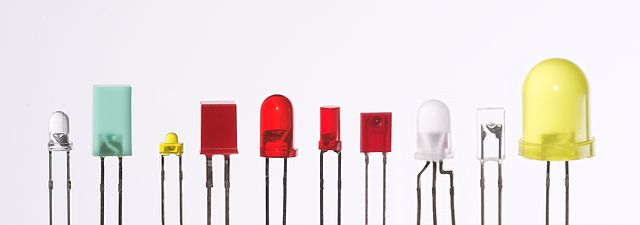
\includegraphics[width=0.8\textwidth,height=.55\textheight,keepaspectratio]{a05/Verschiedene_LEDs.jpg}
        \attribcaption{LEDs in verschiedenen Gehäusen}{Afrank99}{https://commons.wikimedia.org/wiki/File:Verschiedene_LEDs.jpg}{\ccbysa}
      \end{figure}
    \end{center}
    \column{.45\textwidth}
    \begin{itemize}
      \item Leuchtet, wenn in Durchlassrichtung betrieben
      \item Betriebsspannung je nach LED-Farbe von etwa $1.5V$ bis $3.2V$
    \end{itemize}
  \end{columns}
\end{frame}

\subsection*{Optokoppler}
\begin{frame}
  \frametitle{Optokoppler}
  \begin{columns}[c]
    \column[c]{.5\textwidth}
    \begin{center}
      \begin{figure}
        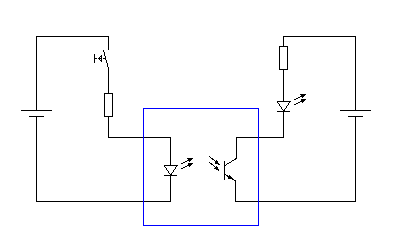
\includegraphics[width=1\textwidth,height=.35\textheight,keepaspectratio]{a05/Optokoppler_Aus.png}\\
        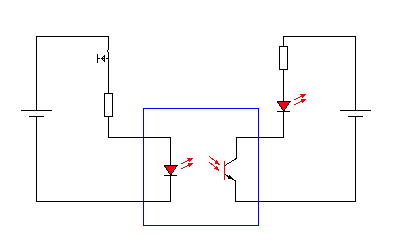
\includegraphics[width=1\textwidth,height=.35\textheight,keepaspectratio]{a05/Optokoppler_An.png}
        \attribcaption{Funktionsprinzip eines Optokopplers (animiertes GIF)}{Stefan Riepl}{http://commons.wikimedia.org/wiki/File:Optokoppler.gif}{\ccbysa}
      \end{figure}
      \tiny \hyperlink{refs}{\cite{wm}}
    \end{center}
    \column{.45\textwidth}
    \begin{itemize}
      \item LED und Photodiode in einem Bauelement
      \item Galvanische Trennung von zwei Schaltkreisen
      \item Probleme bei Hochfrequenzschaltungen
    \end{itemize}
  \end{columns}
\end{frame}

\section*{Anwendungen der Diode}

\subsection*{Spannungs\-begrenzung}
\begin{frame}
  \frametitle{Spannungsbegrenzung}
  \begin{columns}[c]
    \column[c]{.5\textwidth}
    \begin{center}
      \begin{figure}
        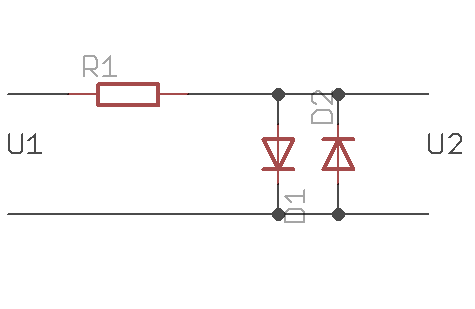
\includegraphics[width=1\textwidth,height=.75\textheight,keepaspectratio]{a05/spannungsBegrenz.png}
        \caption{Dioden zur Spannungsbegrenzung}
      \end{figure}
    \end{center}
    \column{.45\textwidth}
    \begin{itemize}
      \item Schneidet Signale oberhalb und unterhalb der Durchlassspannung ab
      \item Gut als Überspannungsschutz
    \end{itemize}
  \end{columns}
\end{frame}


\subsection*{Entkopplung}
\begin{frame}
  \frametitle{Entkopplung - Prüfungsfrage TC527}
  \begin{columns}[c]
    \column[c]{.5\textwidth}
    \begin{center}
      \begin{figure}
        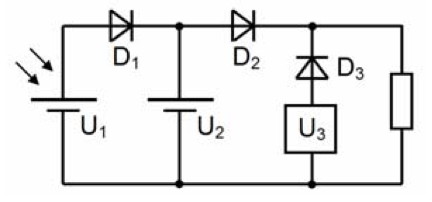
\includegraphics[width=1\textwidth,height=.75\textheight,keepaspectratio]{a05/TC527.png}
        \caption{TC527}
      \end{figure}
    \end{center}
    \column{.45\textwidth}
    Der Sonnenkollektor liefert $U_1 = 14.9V$. \\[0.2em]
    Der Akkumulator hat $U_2 = 13.9V$. \\[0.2em]
    Das Netzteil ist auf $U_3 = 13.5V$ eingestellt. \\[1.2em]
    Welche Dioden leiten und welche nicht?
  \end{columns}
\end{frame}

\section*{Gleichrichter}

\begin{frame}
  \frametitle{Gleichrichter}
  \begin{columns}[c]
    \column[c]{.5\textwidth}
    \begin{center}
      \begin{figure}
        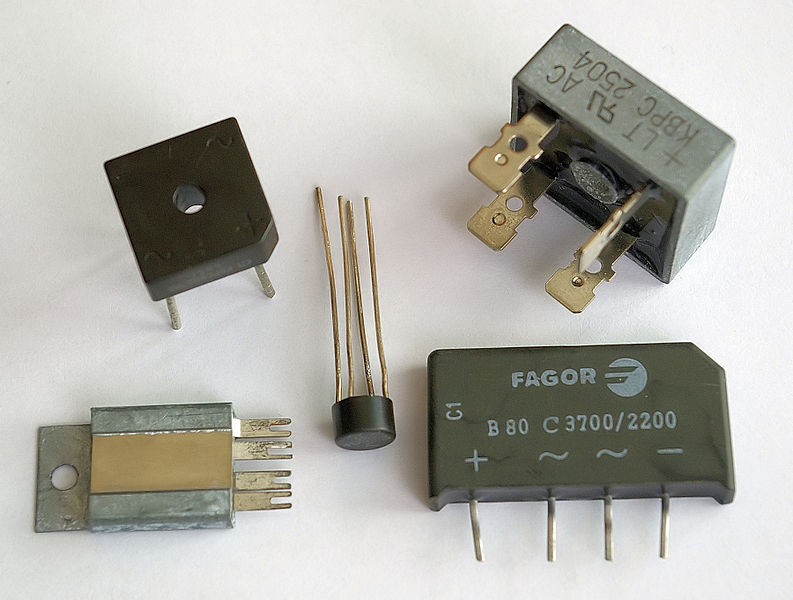
\includegraphics[width=1\textwidth,height=.85\textheight,keepaspectratio]{a05/Brueckengleichrichter_Bilder.jpg}
        \attribcaption{Brückengleichrichter unterschiedlicher Bauformen}{Smial}{https://commons.wikimedia.org/wiki/File:Brueckengleichrichter_IMGP5380.jpg}{\ccbysa}
      \end{figure}
    \end{center}
    \column{.45\textwidth}
    \begin{itemize}
      \item Gleichrichter machen aus Wechselspannung Gleichspannung
      \item Mit Hilfe von Dioden wird die obere und untere Halbwelle getrennt
      \item Ohne Dioden sehr schwierig
    \end{itemize}
  \end{columns}
\end{frame}

\begin{frame}
  \frametitle{Einweggleichrichtung}
  \begin{center}
    \begin{figure}
      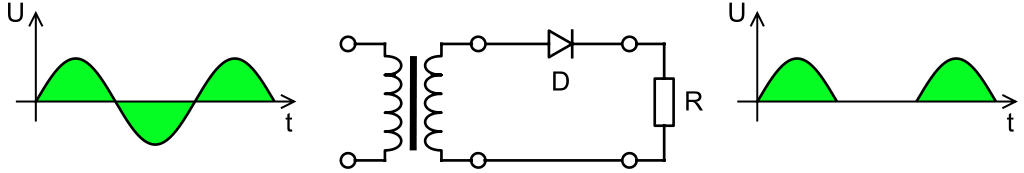
\includegraphics[width=1\textwidth,height=.6\textheight,keepaspectratio]{a05/Halfwave_rectifier.png}
      \attribcaption{Einweggleichrichtung}{Wdwd}{https://commons.wikimedia.org/wiki/File:Halfwave.rectifier.en.svg}{\ccby}
    \end{figure}
    \begin{itemize}
      \item Nur obere Halbwelle, also sehr geringe Ausbeute
      \item Einfach aufzubauen
      \item Wäre mit Kondensator ein AM-Hüllkurvendemodulator (siehe Siebung)
    \end{itemize}
  \end{center}
\end{frame}

\begin{frame}
  \frametitle{Vollweggleichrichtung}
  \begin{center}
    \begin{figure}
      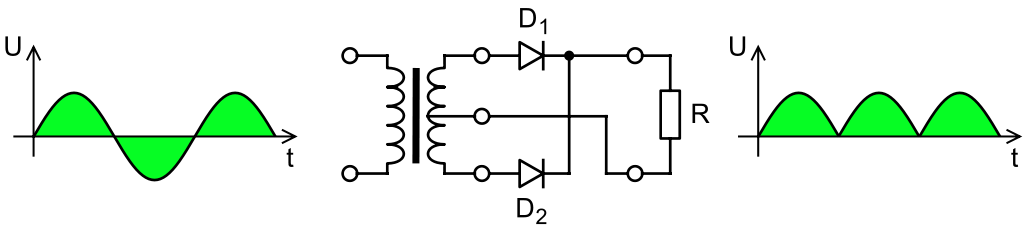
\includegraphics[width=1\textwidth,height=.6\textheight,keepaspectratio]{a05/Fullwave_rectifier.png}
      \attribcaption{Vollweggleichrichtung}{Wdwd}{https://commons.wikimedia.org/wiki/File:Fullwave.rectifier.en.svg}{\ccby}
    \end{figure}
    \begin{itemize}
      \item Obere und untere Halbwelle, also deutlich mehr Ausbeute
      \item Schwieriger aufzubauen
      \item Verdoppelt die Abtastrate
      \item Benötigt Transformator mit Mittelpunktanzapfung (siehe \href{https://commons.wikimedia.org/wiki/File:Gleichrichter_mittelanzapfg_ani.gif}{\ExternalLink animierte Grafik})
    \end{itemize}
  \end{center}
\end{frame}

\begin{frame}
  \frametitle{Brückengleichrichtung}
  \begin{center}
    \begin{figure}
      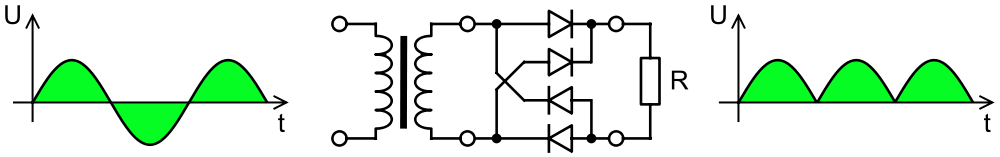
\includegraphics[width=1\textwidth,height=.6\textheight,keepaspectratio]{a05/Gratz_rectifier.png}
      \attribcaption{Grätz (Brücken-)Gleichrichter}{Wdwd}{https://commons.wikimedia.org/wiki/File:Gratz.rectifier.en.svg}{\ccby}
    \end{figure}
    \begin{itemize}
      \item Obere und untere Halbwelle, also deutlich mehr Ausbeute
      \item Schwieriger aufzubauen
      \item Verdoppelt Frequenz
      \item Benötigt vier Dioden
    \end{itemize}
  \end{center}
\end{frame}

\begin{frame}
  \frametitle{Siebung}
  \begin{columns}[c]
    \column[c]{.5\textwidth}
    \begin{center}
      \begin{figure}
        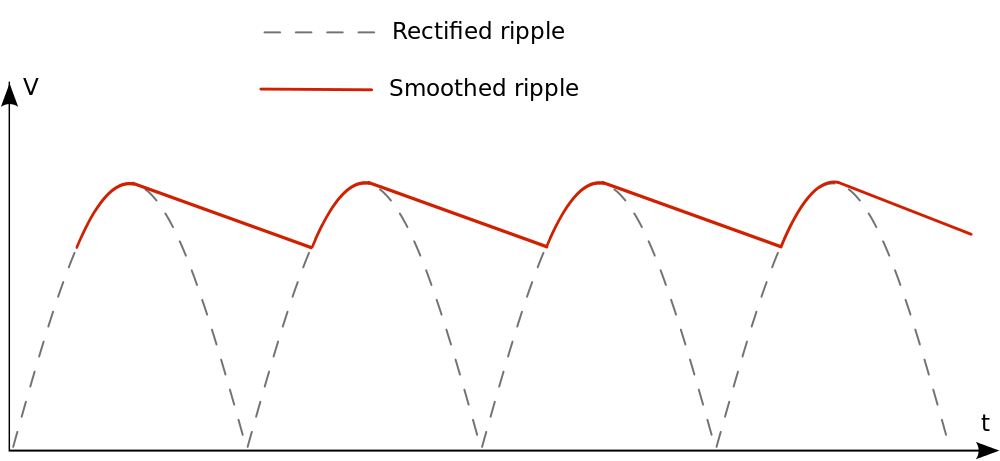
\includegraphics[width=1\textwidth,height=.75\textheight,keepaspectratio]{a05/Smoothed_ripple.png}
        \attribcaption{Restwelligkeit (rot) einer gleichgerichteten Wechselspannung (grau gestrichelt).}{SpinningSpark}{https://commons.wikimedia.org/wiki/File:Smoothed_ripple.svg}{\ccbysa}
      \end{figure}
    \end{center}
    \column{.45\textwidth}
    \begin{itemize}
      \item Glättung durch Tiefpass hinter dem Gleichrichter
      \item Durch verdoppelte Frequenz noch einfacher umzusetzen
      \item LC-TP oder RC-TP nutzbar
      \item In der Realität oft Elektrolytkondensatoren mit mehreren $mF$
    \end{itemize}
  \end{columns}
\end{frame}

\begin{frame}
  \begin{tabular}{l|p{.8\textwidth}}\hline
    \textbf{TF317} &
    \begin{tabular}{c}
      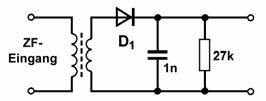
\includegraphics[width=\textwidth,height=.5\textheight,keepaspectratio]{a05/tf317.png}
    \end{tabular}
    \textbf{Bei der Schaltung handelt es sich um einen... ?}
  \end{tabular}
\end{frame}

\begin{frame}
  \frametitle{Gleichspannungsrückgewinnung}
  \begin{center}
    \begin{figure}
      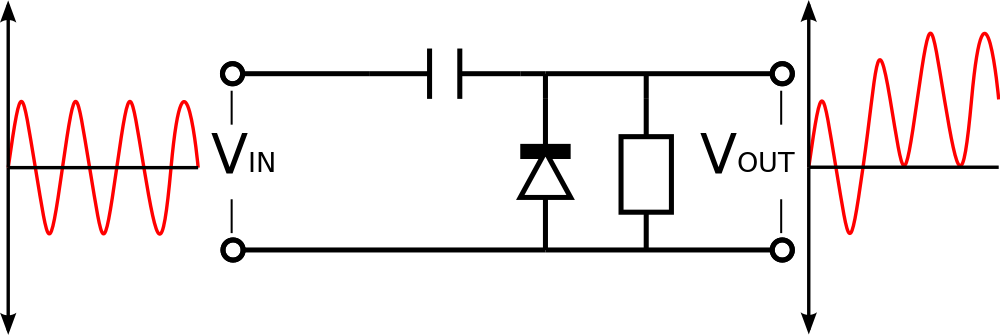
\includegraphics[width=1\textwidth,height=.6\textheight,keepaspectratio]{a05/Positive_Voltage_Clamping_Circuit.png}
      \attribcaption{Positive voltage clamping circuit}{Jack1993jack}{https://en.wikipedia.org/wiki/File:Positive_Voltage_Clamping_Circuit.svg}{\ccbysa}
    \end{figure}
    \begin{itemize}
      \item Wird benutzt um das Signal anzuheben
      \item Wird z.B. bei Verstärkerschaltungen benötigt
    \end{itemize}
  \end{center}
\end{frame}

\renewcommand{\refname}{Referenzen}

\hypertarget{refs}{}
\textcolor{white}{} \\ %\vspace{} geht nicht
\Large Referenzen/Links
\footnotesize

\begin{thebibliography}{}
  \bibitem{darc}  DARC Online-Lehrgang Lektion A05:
    \url{https://www.darc.de/der-club/referate/ajw/lehrgang-ta/a05/}
  \bibitem{wp}    Wikipedia - Die freie Enzyklopädie:
    \url{https://de.wikipedia.org/wiki/Gleichrichter}
  \bibitem{bna}   Fragenkatalog Bundesnetzagentur Technik Klasse A:
    \url{https://www.bundesnetzagentur.de/SharedDocs/Downloads/DE/Sachgebiete/Telekommunikation/Unternehmen_Institutionen/Frequenzen/Amateurfunk/Fragenkatalog/TechnikFragenkatalogKlasseAf252rId9014pdf.pdf?__blob=publicationFile&v=3}
  \bibitem{fi}    Freie Inhalte (DK0TU):
    \url{https://www.dk0tu.de/Projekte/Freie_Inhalte/}
\end{thebibliography}

% Hier könnte noch eine Kontaktfolie stehen

\end{document}

